\section{Typische Versuchsstände und Aufgaben}

\subsection{Typische Versuchsstände}

\begin{figure}[h!]
	\begin{minipage}[b]{.4\textwidth} % [b] => Ausrichtung an \caption
		\centering
		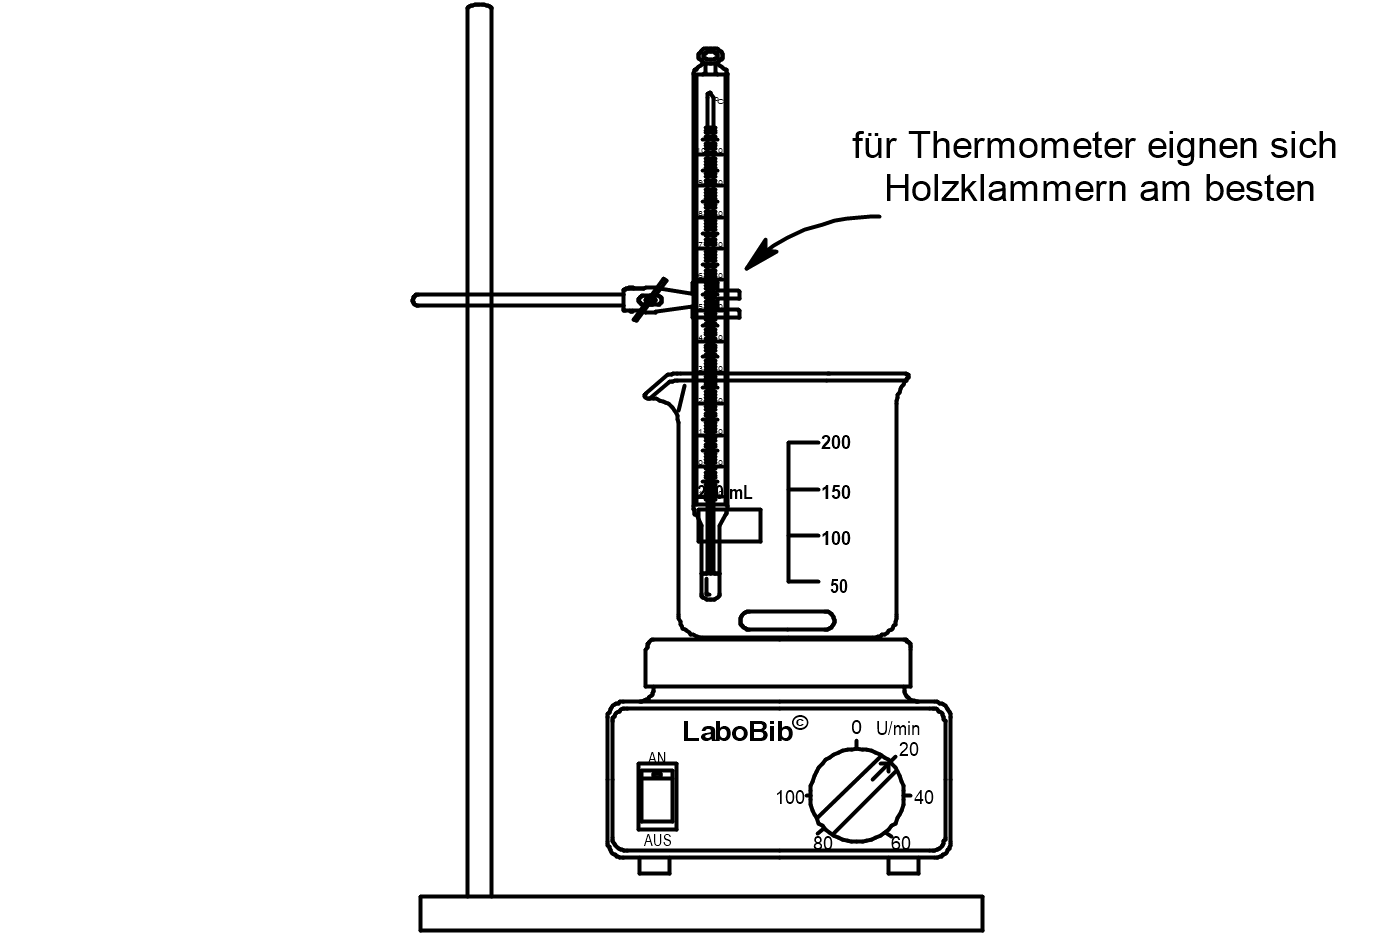
\includegraphics[width=1.3\textwidth]{img/versuchsstand/becherglas_ruehr2}
		\caption{Becherglas-Rührapparatur}
		\label{fig:becherglas_ruehrapparatur}
	\end{minipage}
	\hspace{.1\linewidth}% Abstand zwischen Bilder
	\begin{minipage}[b]{.4\textwidth} % [b] => Ausrichtung an \caption
		\centering
		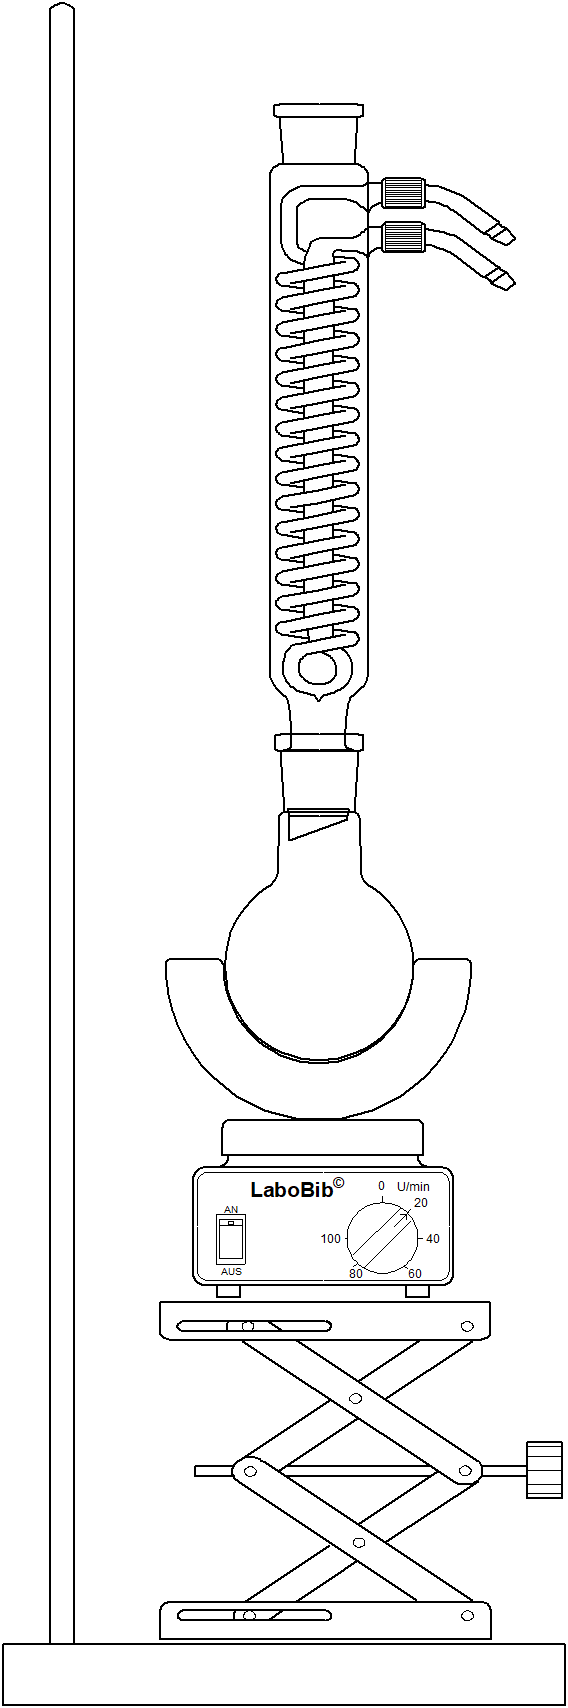
\includegraphics[width=0.4\textwidth]{img/versuchsstand/ruckfluss}
		\caption{Rückflussapparatur}
		\label{fig:ruckfluss}
	\end{minipage}
\end{figure}
\FloatBarrier

\begin{figure}[h!]
	\begin{minipage}[b]{.45\textwidth} % [b] => Ausrichtung an \caption
		\centering
		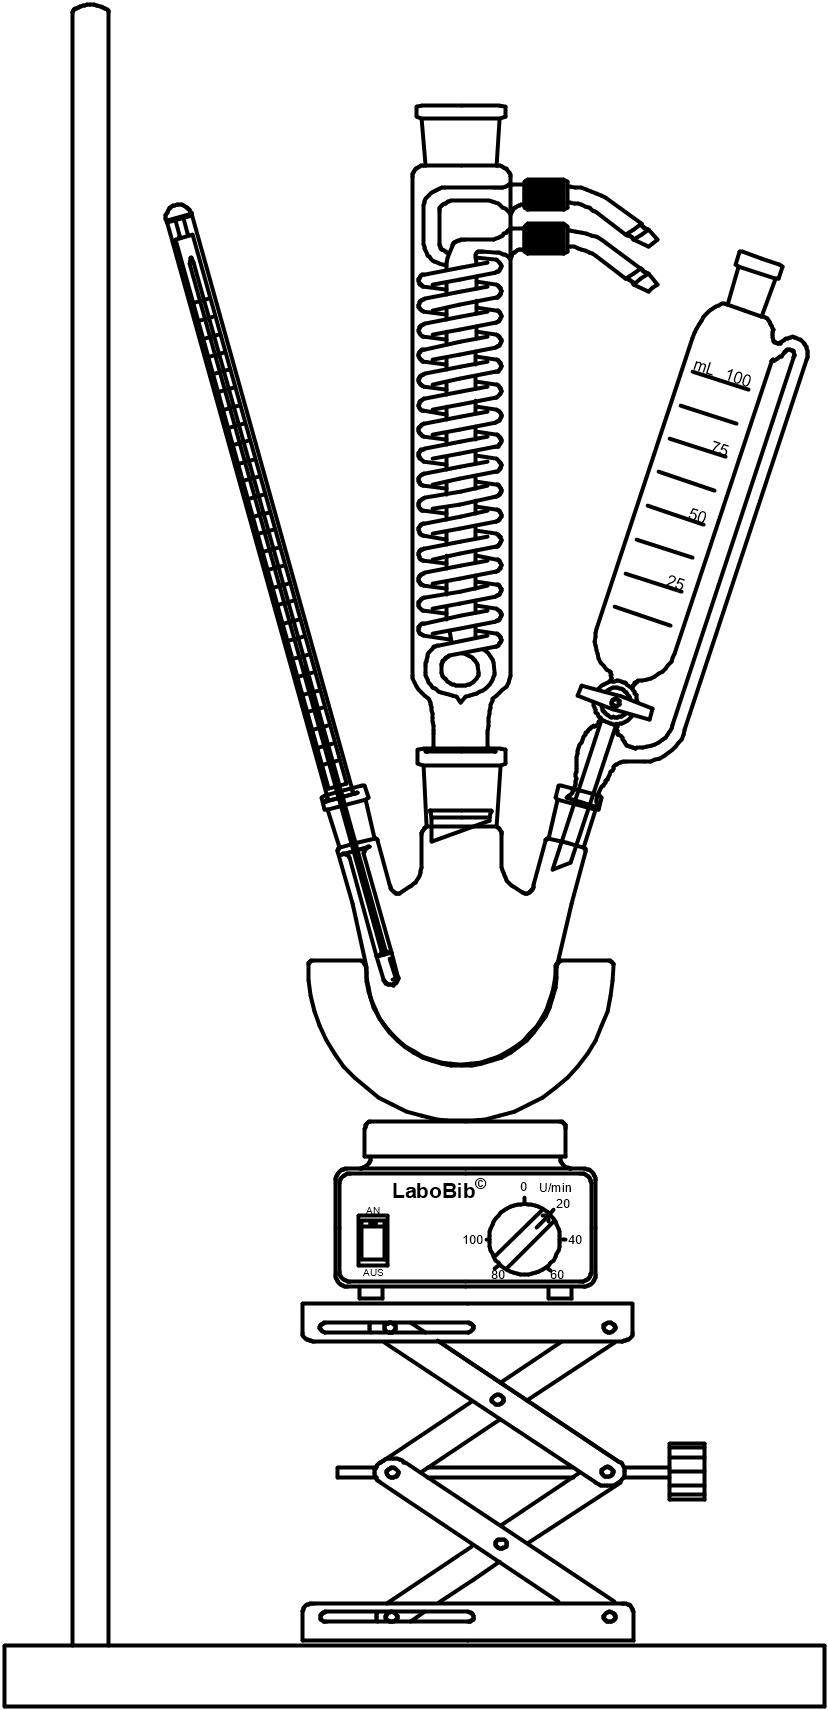
\includegraphics[width=0.5\textwidth]{img/versuchsstand/dreihals}
		\caption{Mehrhalskolbenapparatur}
		\label{fig:mehrhals}
	\end{minipage}
\hspace{.1\linewidth}% Abstand zwischen Bilder
\begin{minipage}[b]{.45\textwidth} % [b] => Ausrichtung an \caption
	\centering
	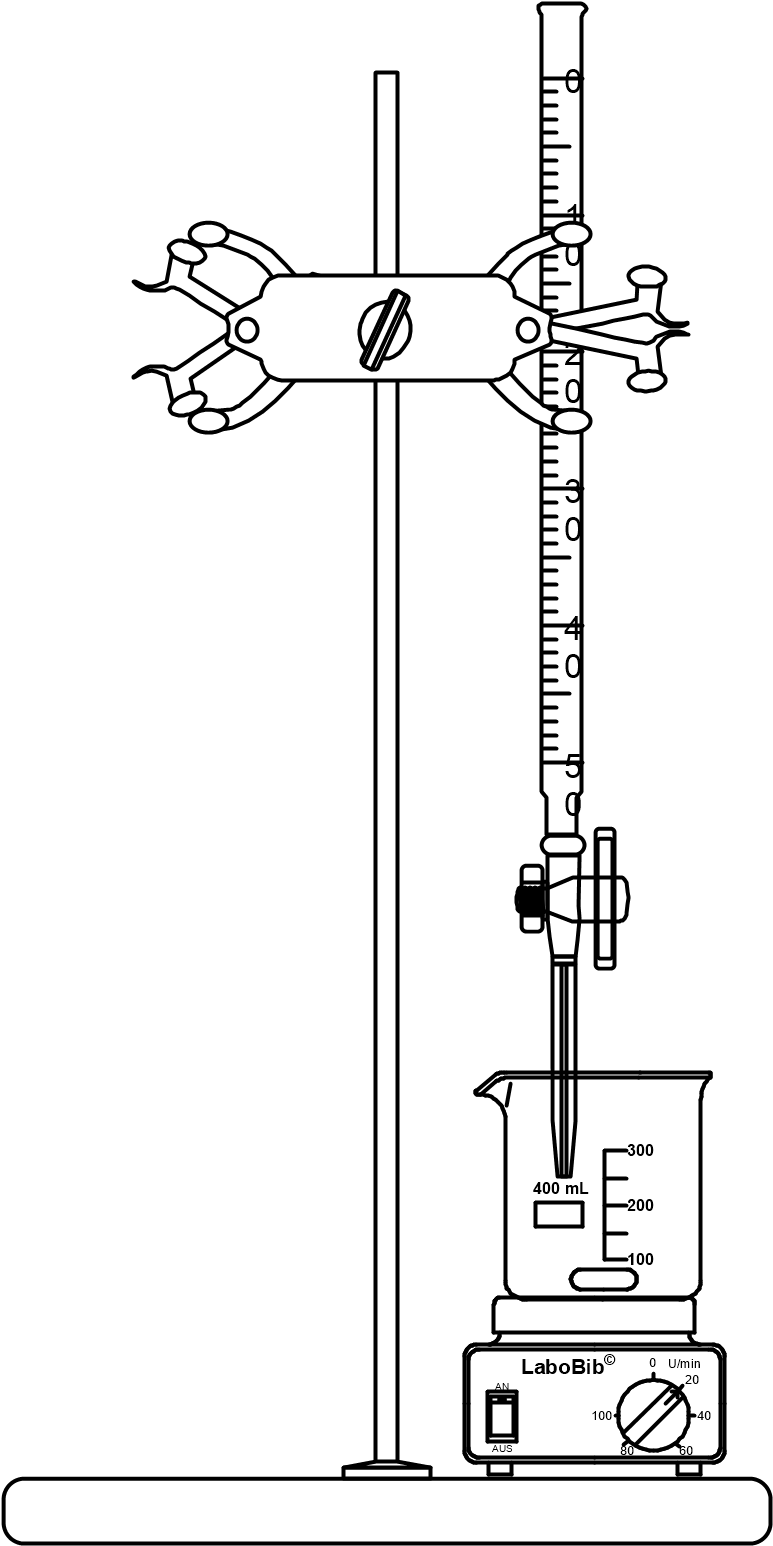
\includegraphics[width=0.5\textwidth]{img/versuchsstand/titration}
	\caption{Titrationsapparatur}
	\label{fig:titration}
\end{minipage}
\end{figure}
\FloatBarrier

\newpage

\subsection{Typische Verfahren und Aufgabenstellungen}
\subsubsection*{Dichtebestimmung}
%Start
\begin{figure}[h!]
	\centering
	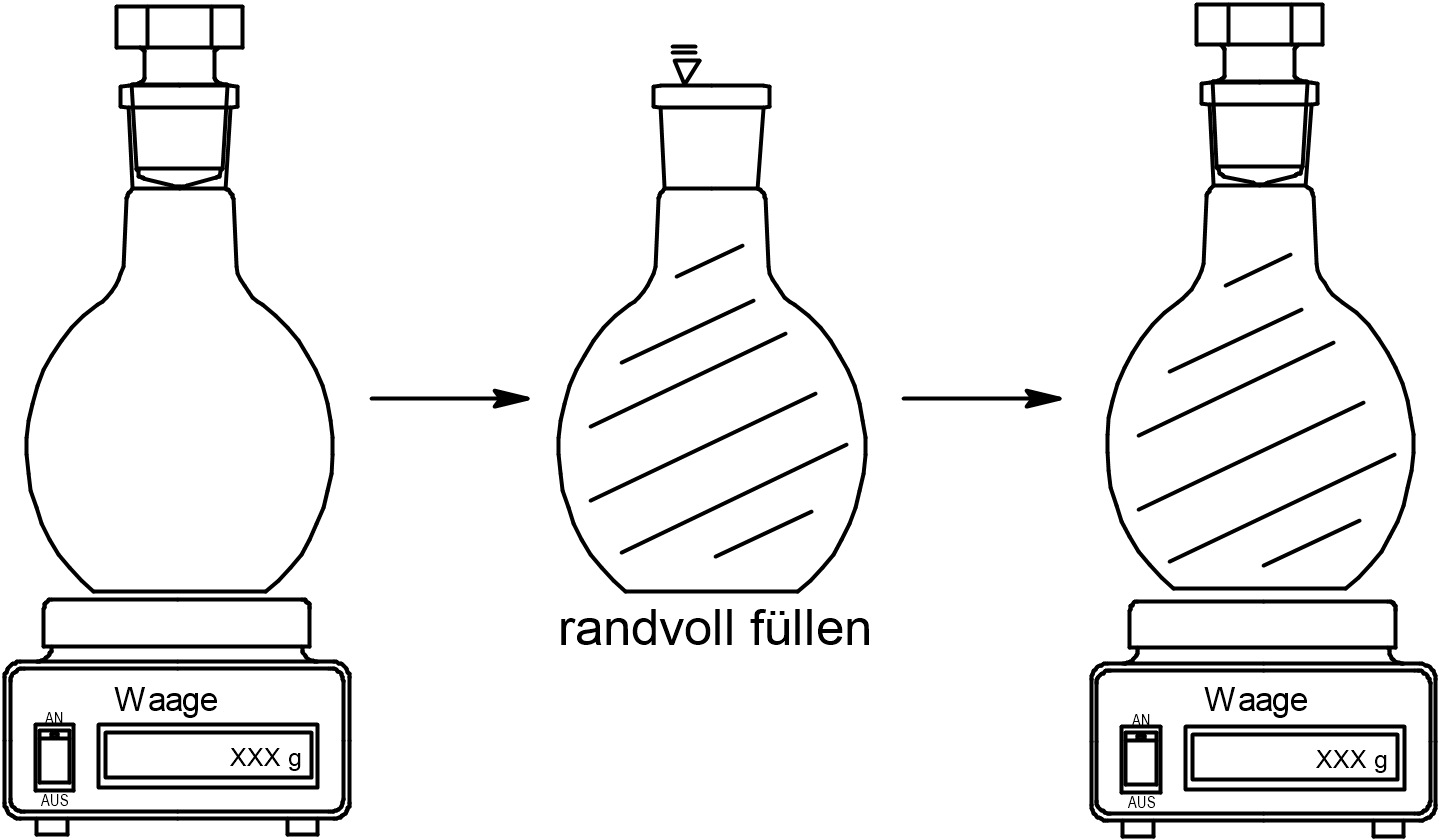
\includegraphics[width=0.4\textwidth]{img/versuchsstand/dichtebestimmung}
	\caption{Dichtebestimmung mittels Pyknometer}
	\label{fig:dichte}
\end{figure}
\FloatBarrier
%Ende

\subsubsection*{Trocknung von Feststoffen}
%Start
\begin{figure}[h!]
	\centering
	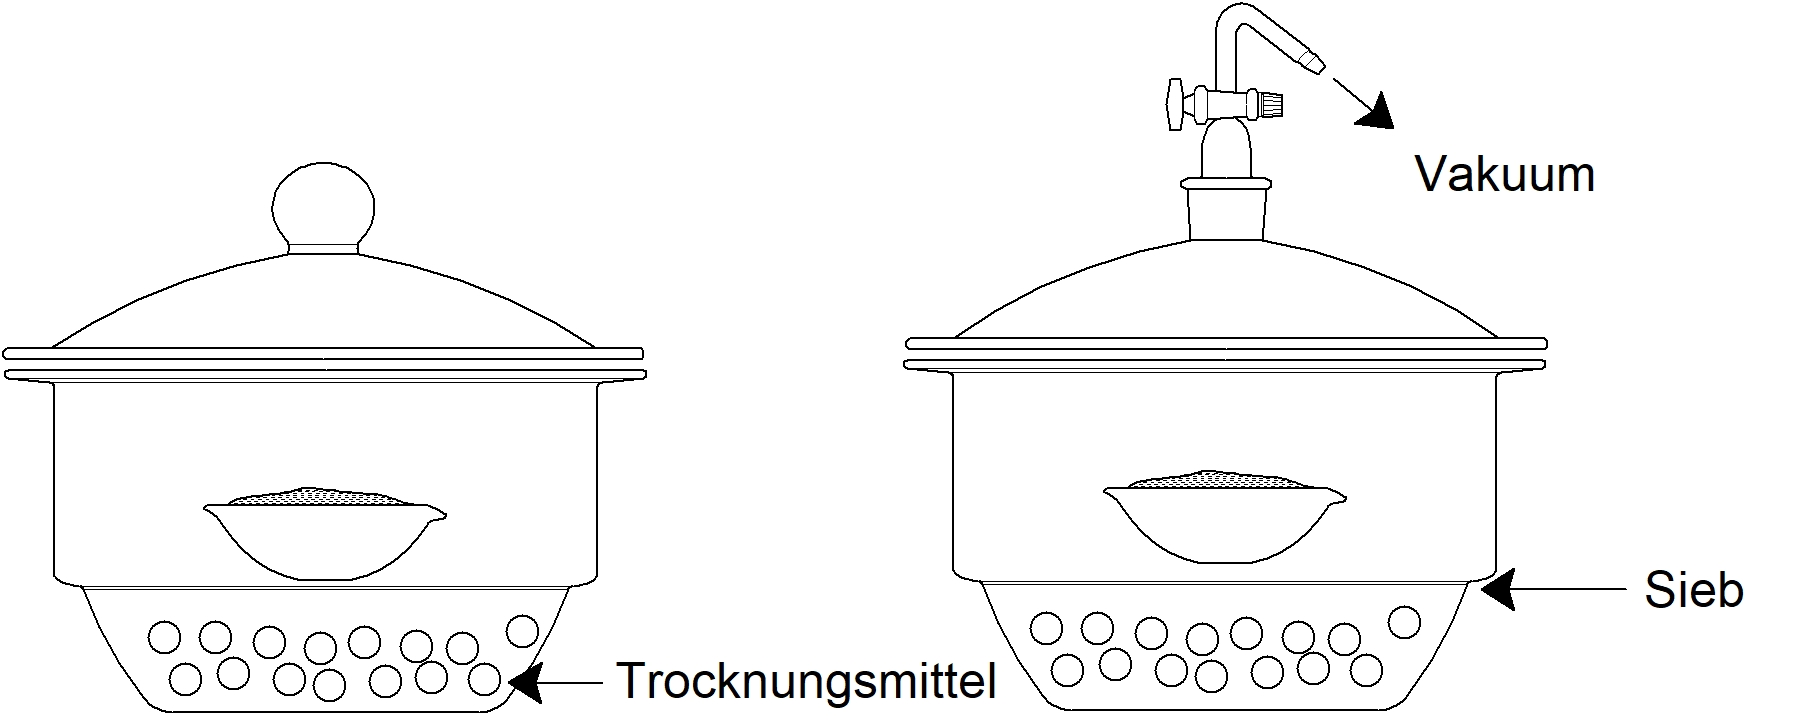
\includegraphics[width=0.75\textwidth]{img/versuchsstand/exsikkator}
	\caption{Trocknung mittels Exsikkator}
	\label{fig:trocknung}
\end{figure}
\FloatBarrier
%Ende

\subsubsection*{Destillation}
%Start
\begin{figure}[h!]
	\centering
	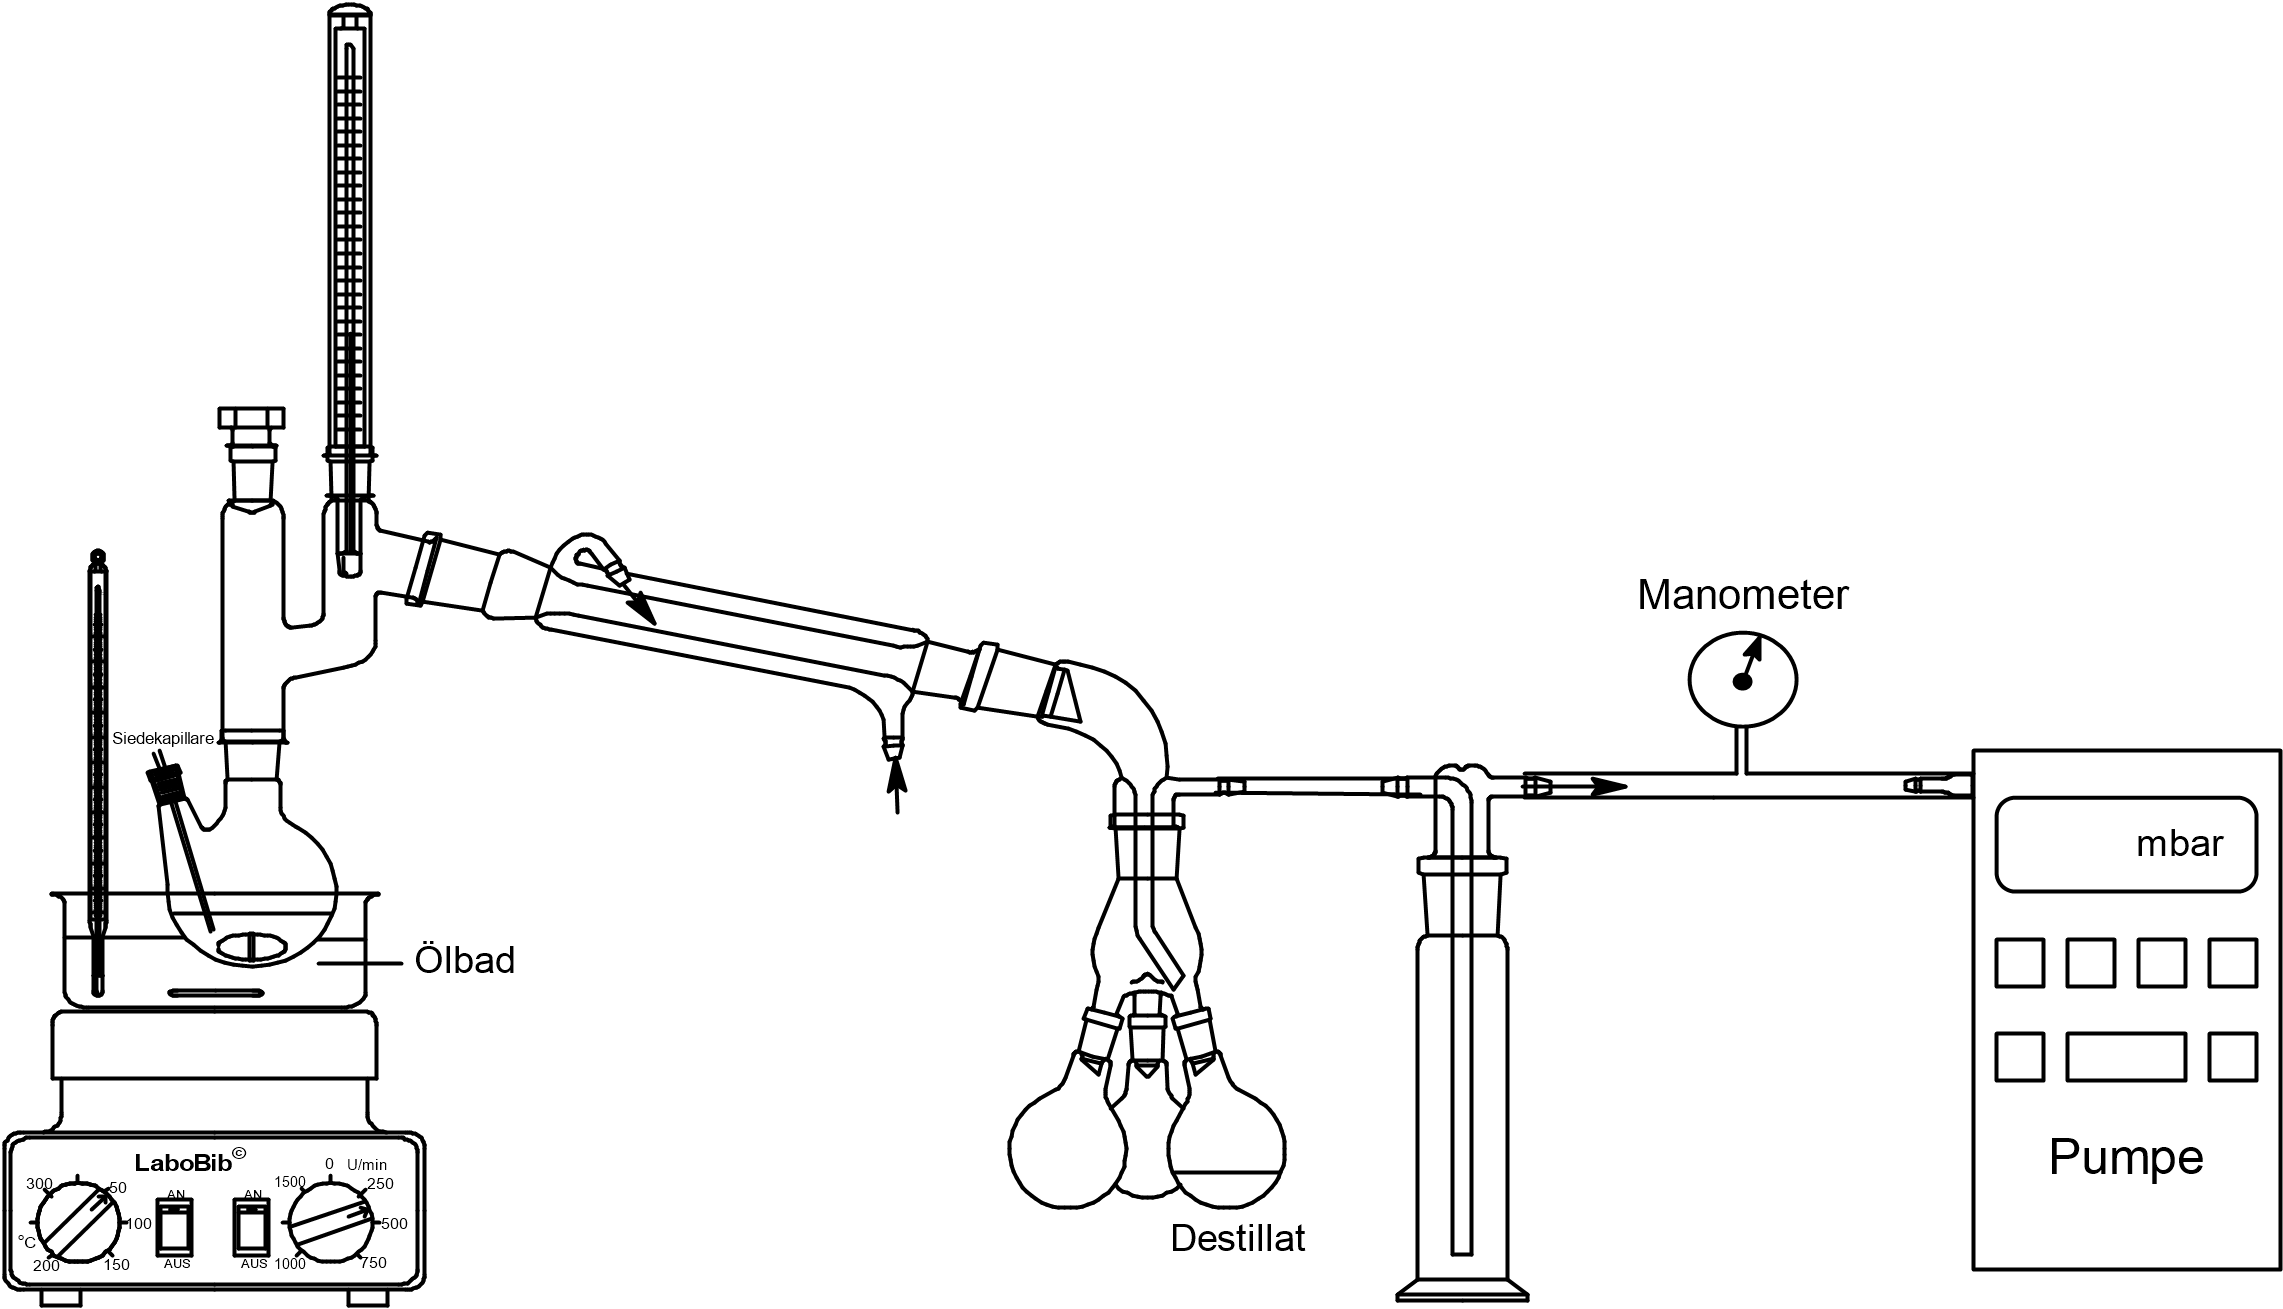
\includegraphics[width=0.75\textwidth]{img/versuchsstand/destillation}
	\caption{Destillationsapparatur}
	\label{fig:destillation}
\end{figure}
\FloatBarrier
%Ende

\subsubsection*{Umkristallisieren}
%Start
\begin{figure}[h!]
	\centering
	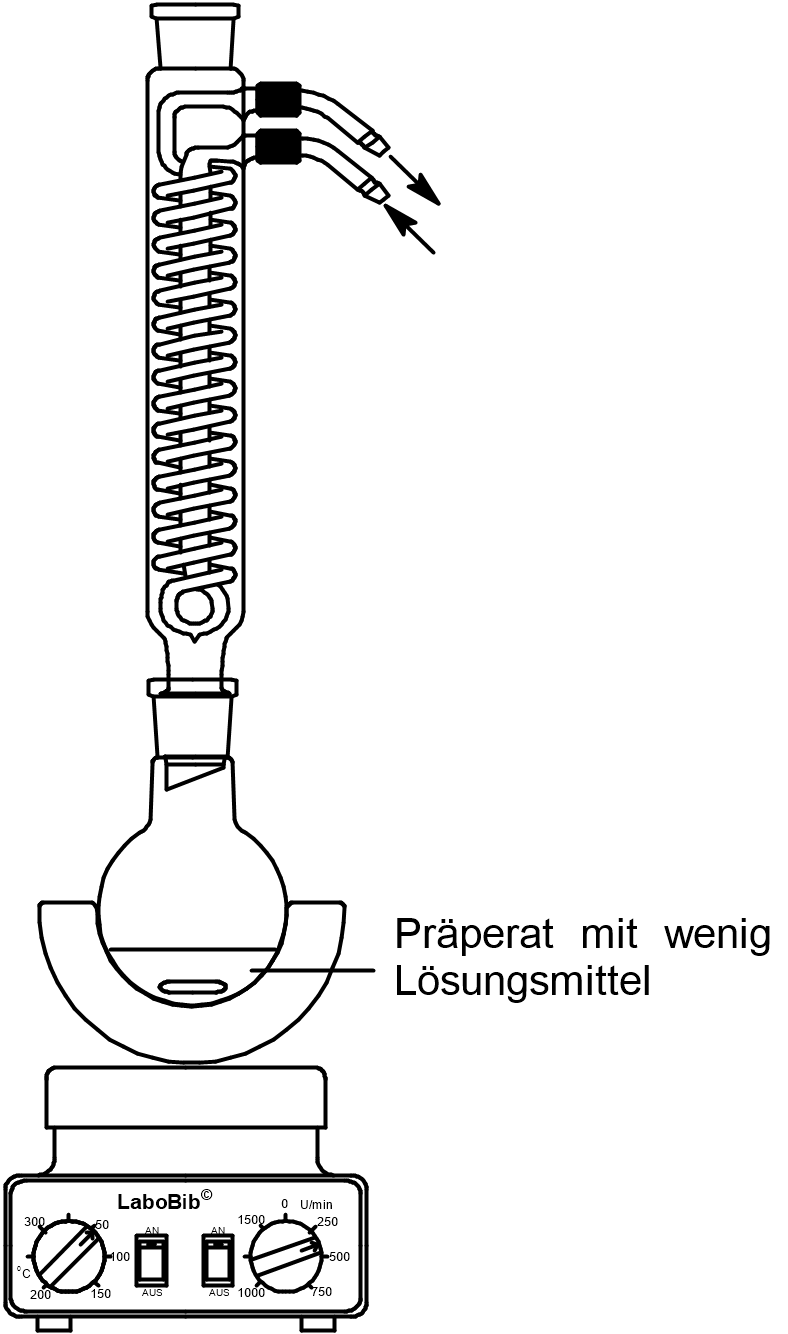
\includegraphics[width=0.2\textwidth]{img/versuchsstand/umkristallisieren}
	\caption{Umkristallisation}
	\label{fig:umkristallisieren}
\end{figure}
\FloatBarrier
%Ende
%http://www.stalke.chemie.uni-goettingen.de/virtuelles_labor/basics/9_more_de.html

\subsubsection*{Extraktion}
\label{sec:extraktion}
%Start
\begin{figure}[h!]
	\centering
	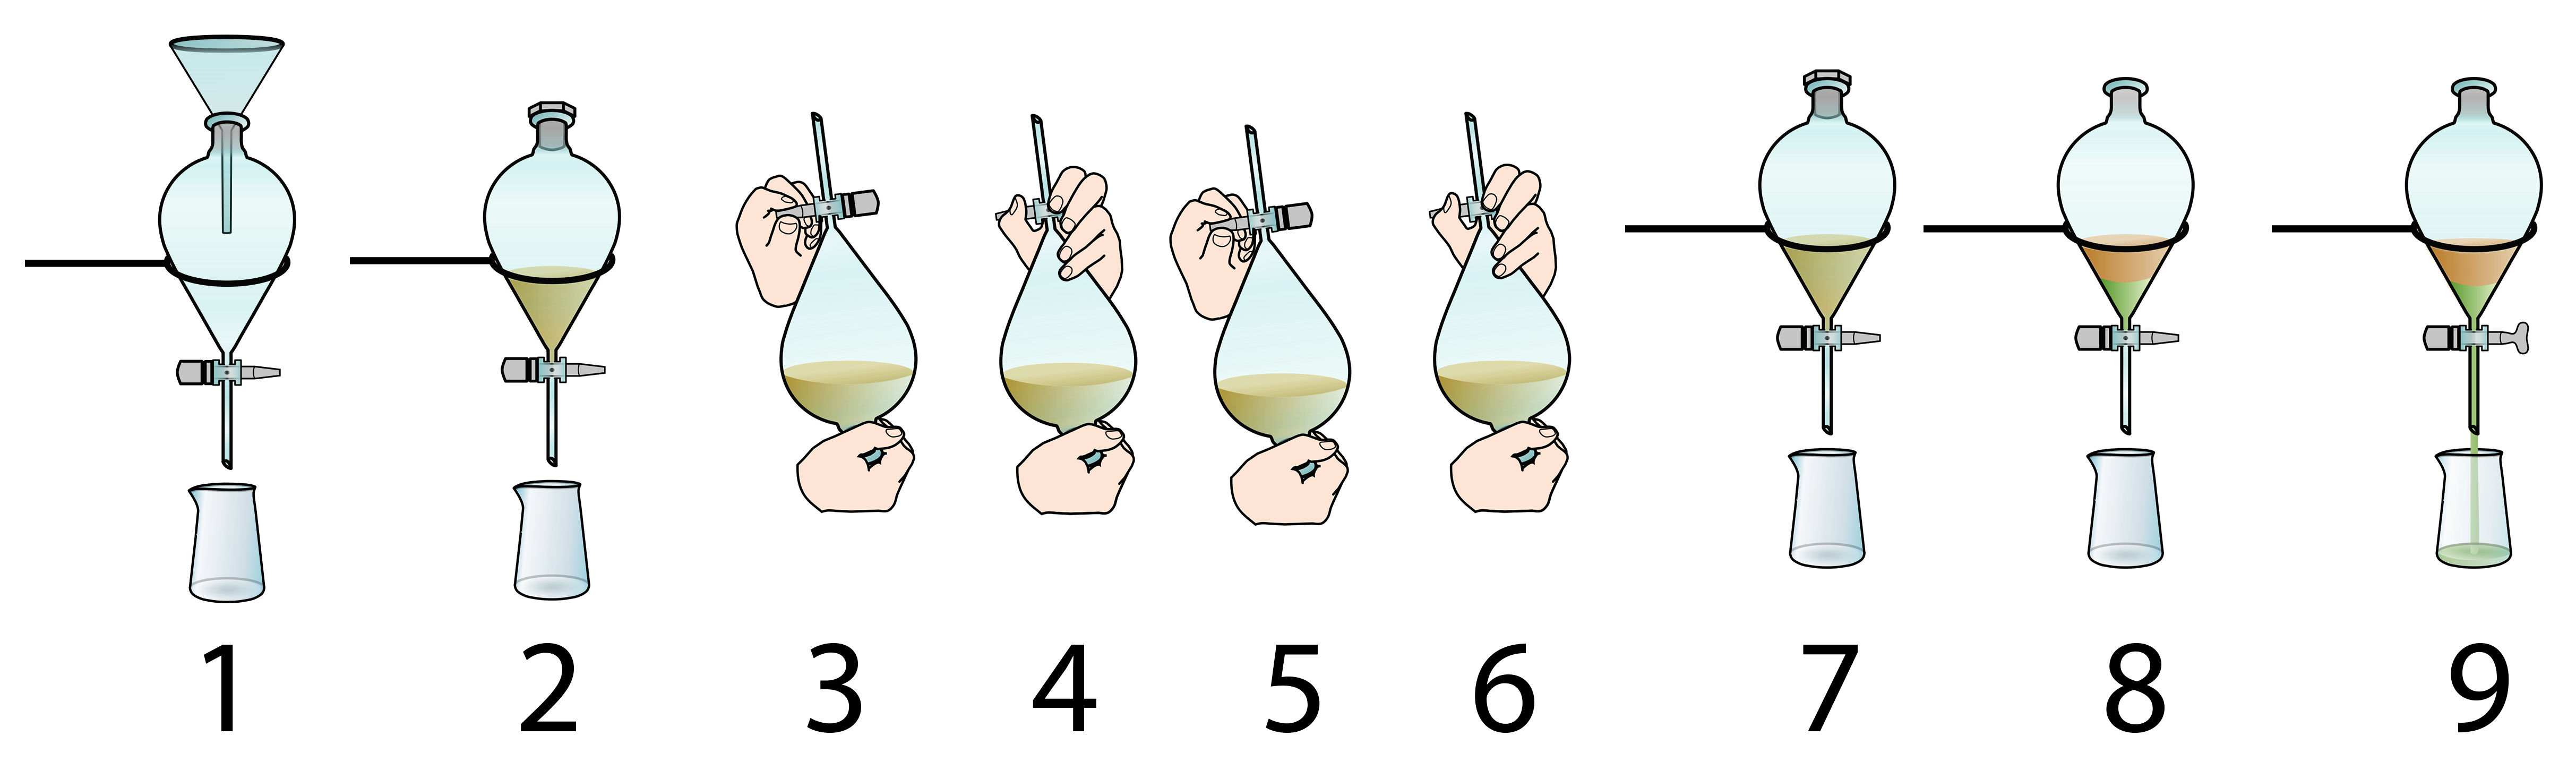
\includegraphics[width=0.9\textwidth]{img/versuchsstand/extraktion}
	\caption{Umkristallisation}
	\label{fig:extraktion}
\end{figure}
\FloatBarrier
%Ende
Auschütteln erklären, Tipp mit gesättigter NaCL Lösung bei Organik

\subsubsection*{Absaugen alias Vakuumfiltrieren}
%Start
\begin{figure}[h!]
	\centering
	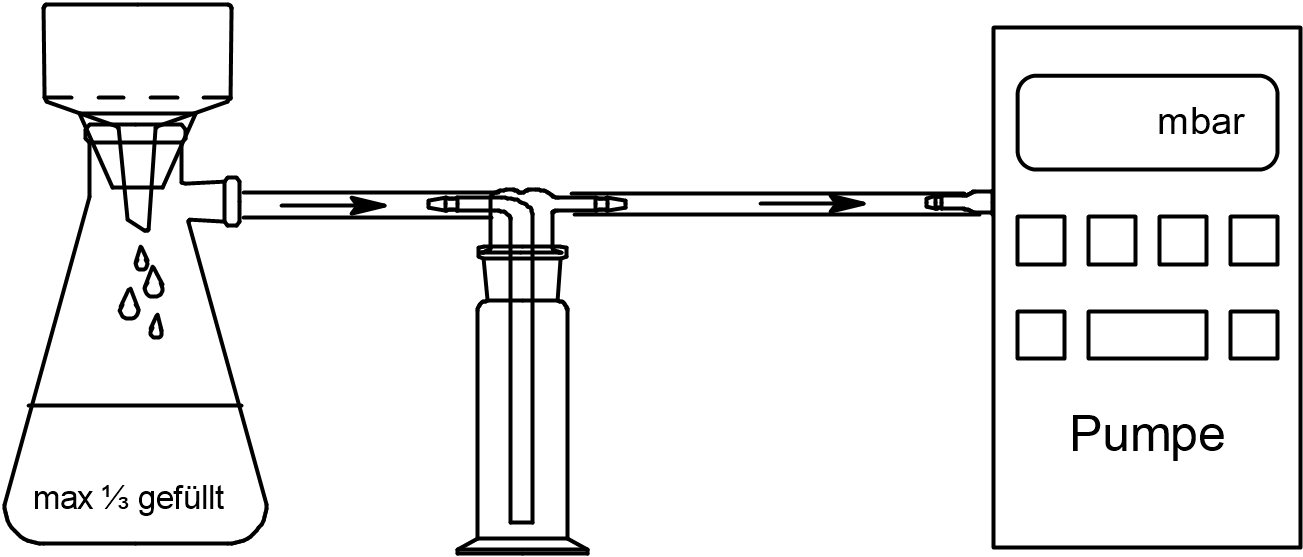
\includegraphics[width=0.5\textwidth]{img/versuchsstand/vakuumfiltration}
	\caption{Apparatur zur Vakuumfiltration}
	\label{fig:vakuumfiltrieren}
\end{figure}
\FloatBarrier
%Ende

\subsubsection*{Schmelzpunkt}
%Start
\begin{figure}[h!]
	\centering
	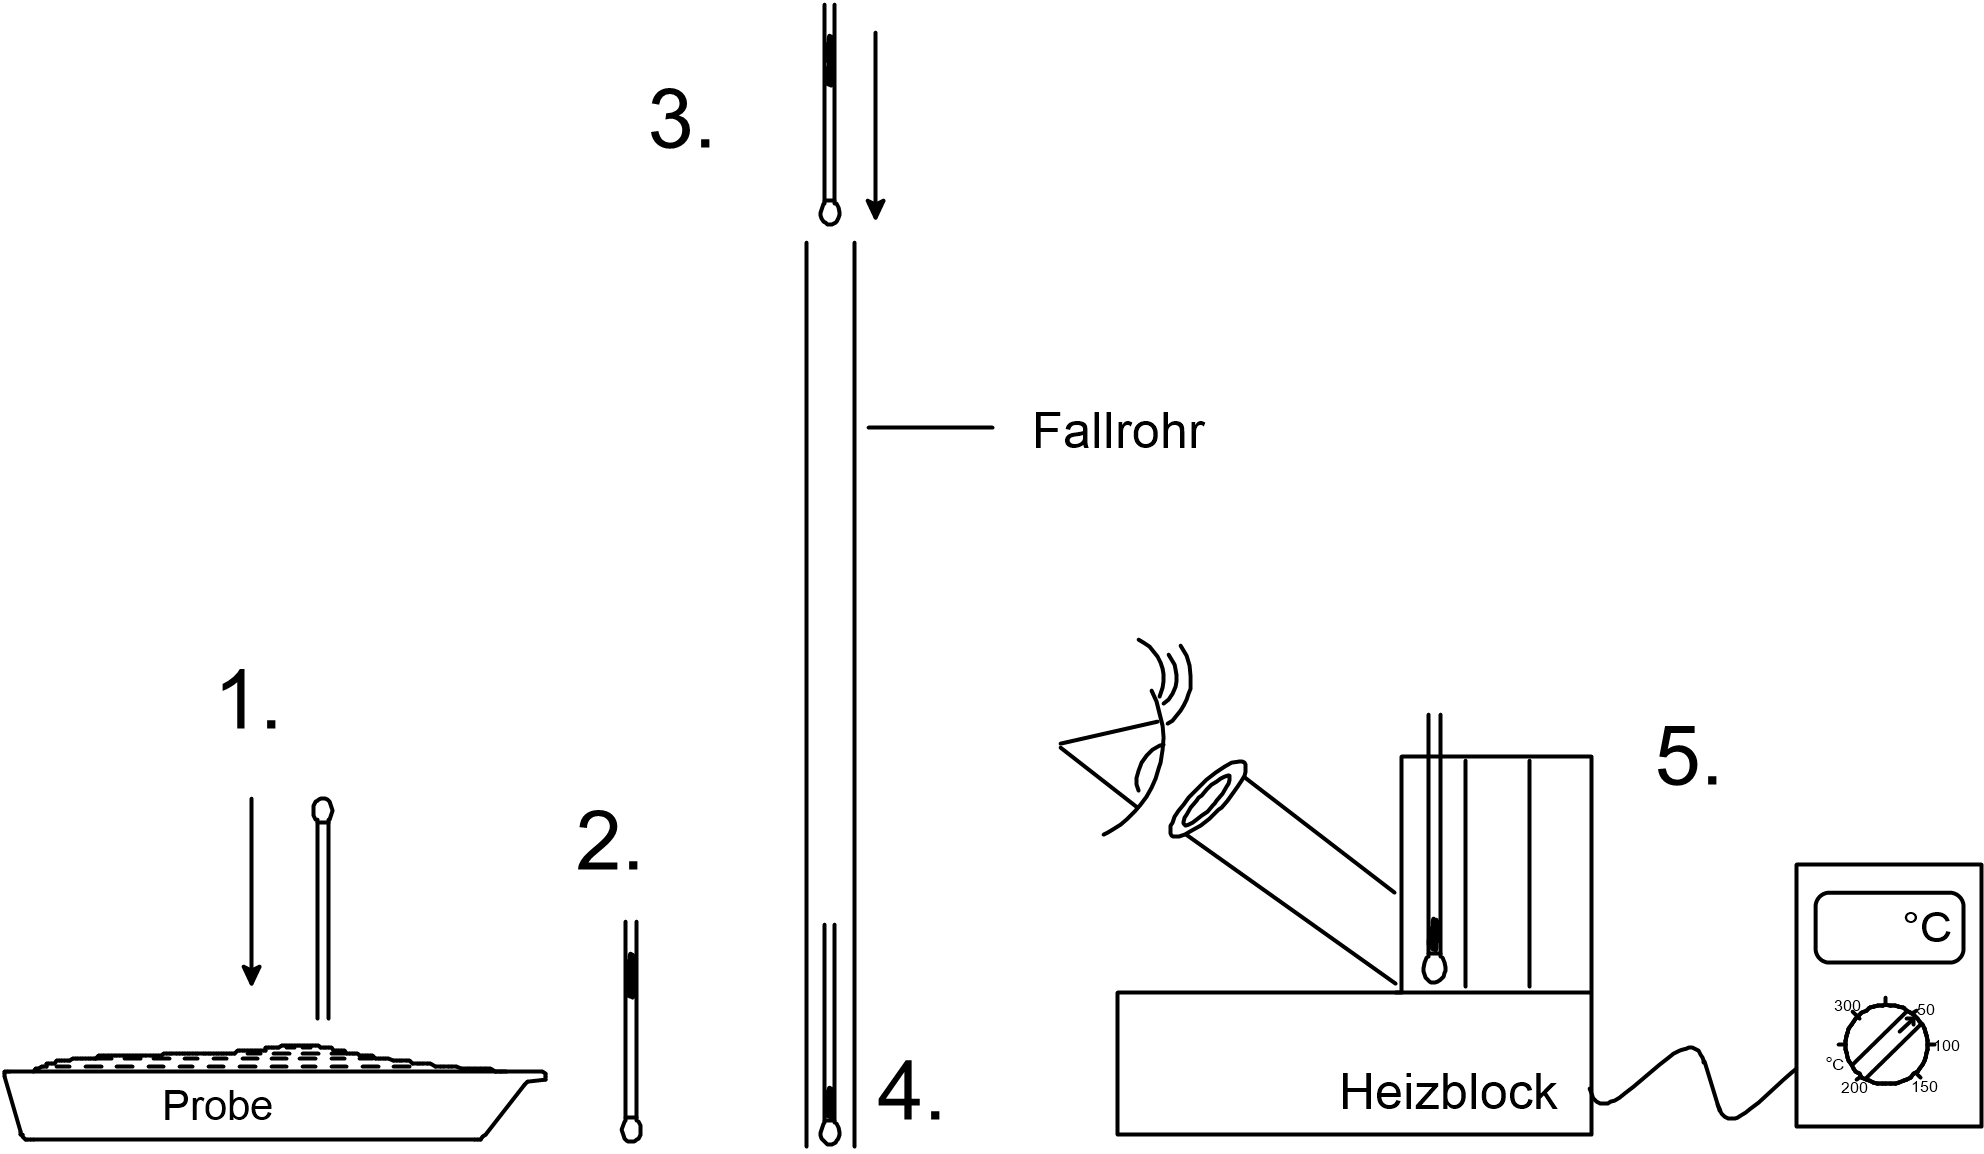
\includegraphics[width=0.7\textwidth]{img/versuchsstand/schmelzpunkt}
	\caption{Schmelzpunktbestimmung mittels Kapillarmethode}
	\label{fig:schmelzpunkt}
\end{figure}
\FloatBarrier
%Ende

\subsubsection*{Siedepunkt}
%Start
\begin{figure}[h!]
	\centering
	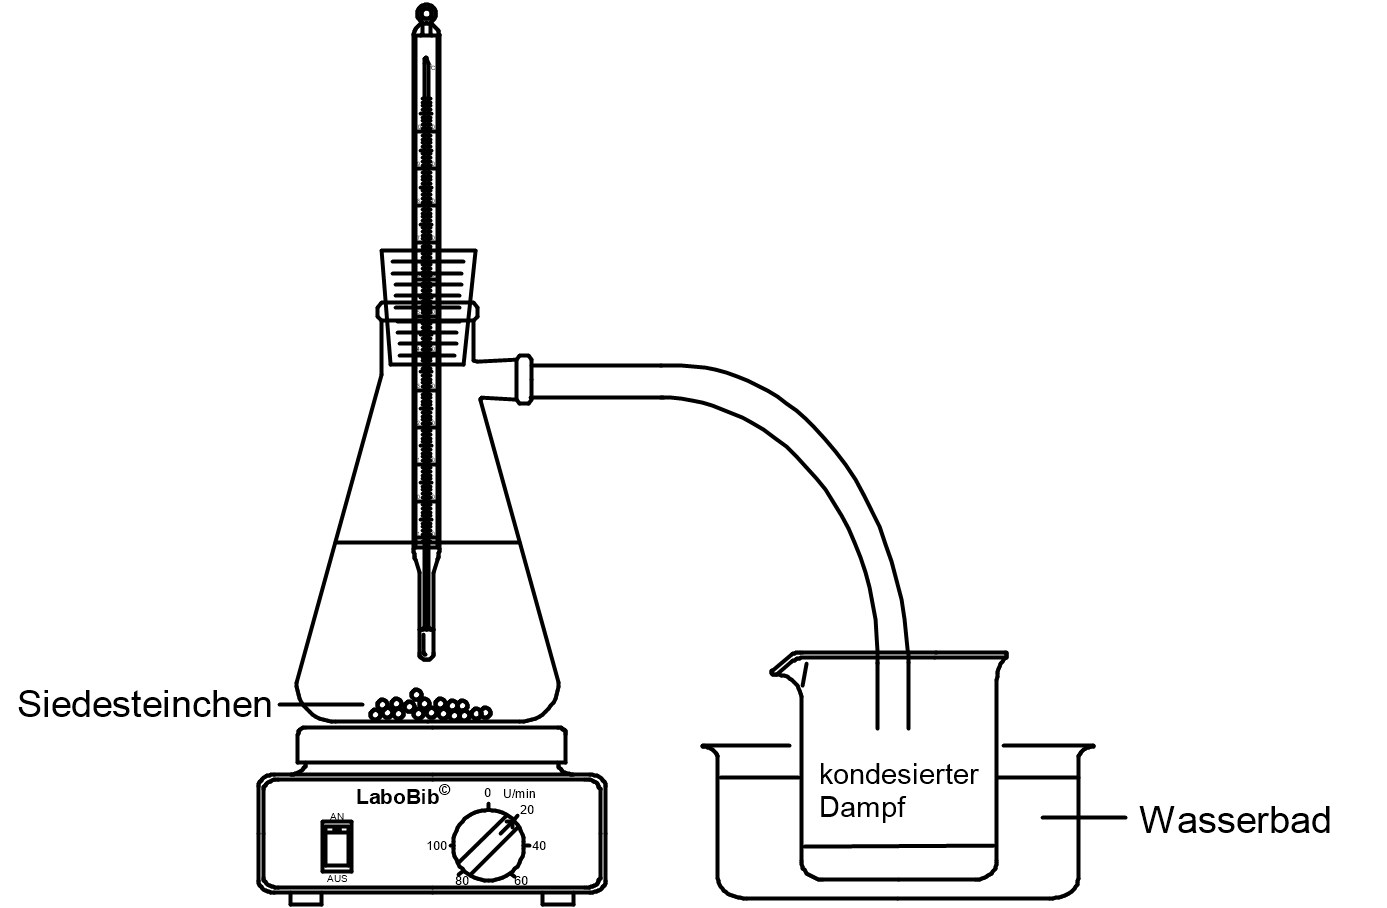
\includegraphics[width=0.5\textwidth]{img/versuchsstand/siedepunkt}
	\caption{simple Siedepunktsbestimmung}
	\label{fig:siedepunkt}
\end{figure}
\FloatBarrier
%Ende

\subsubsection*{Refraktometrie}
%Start
\begin{figure}[h!]
	\centering
	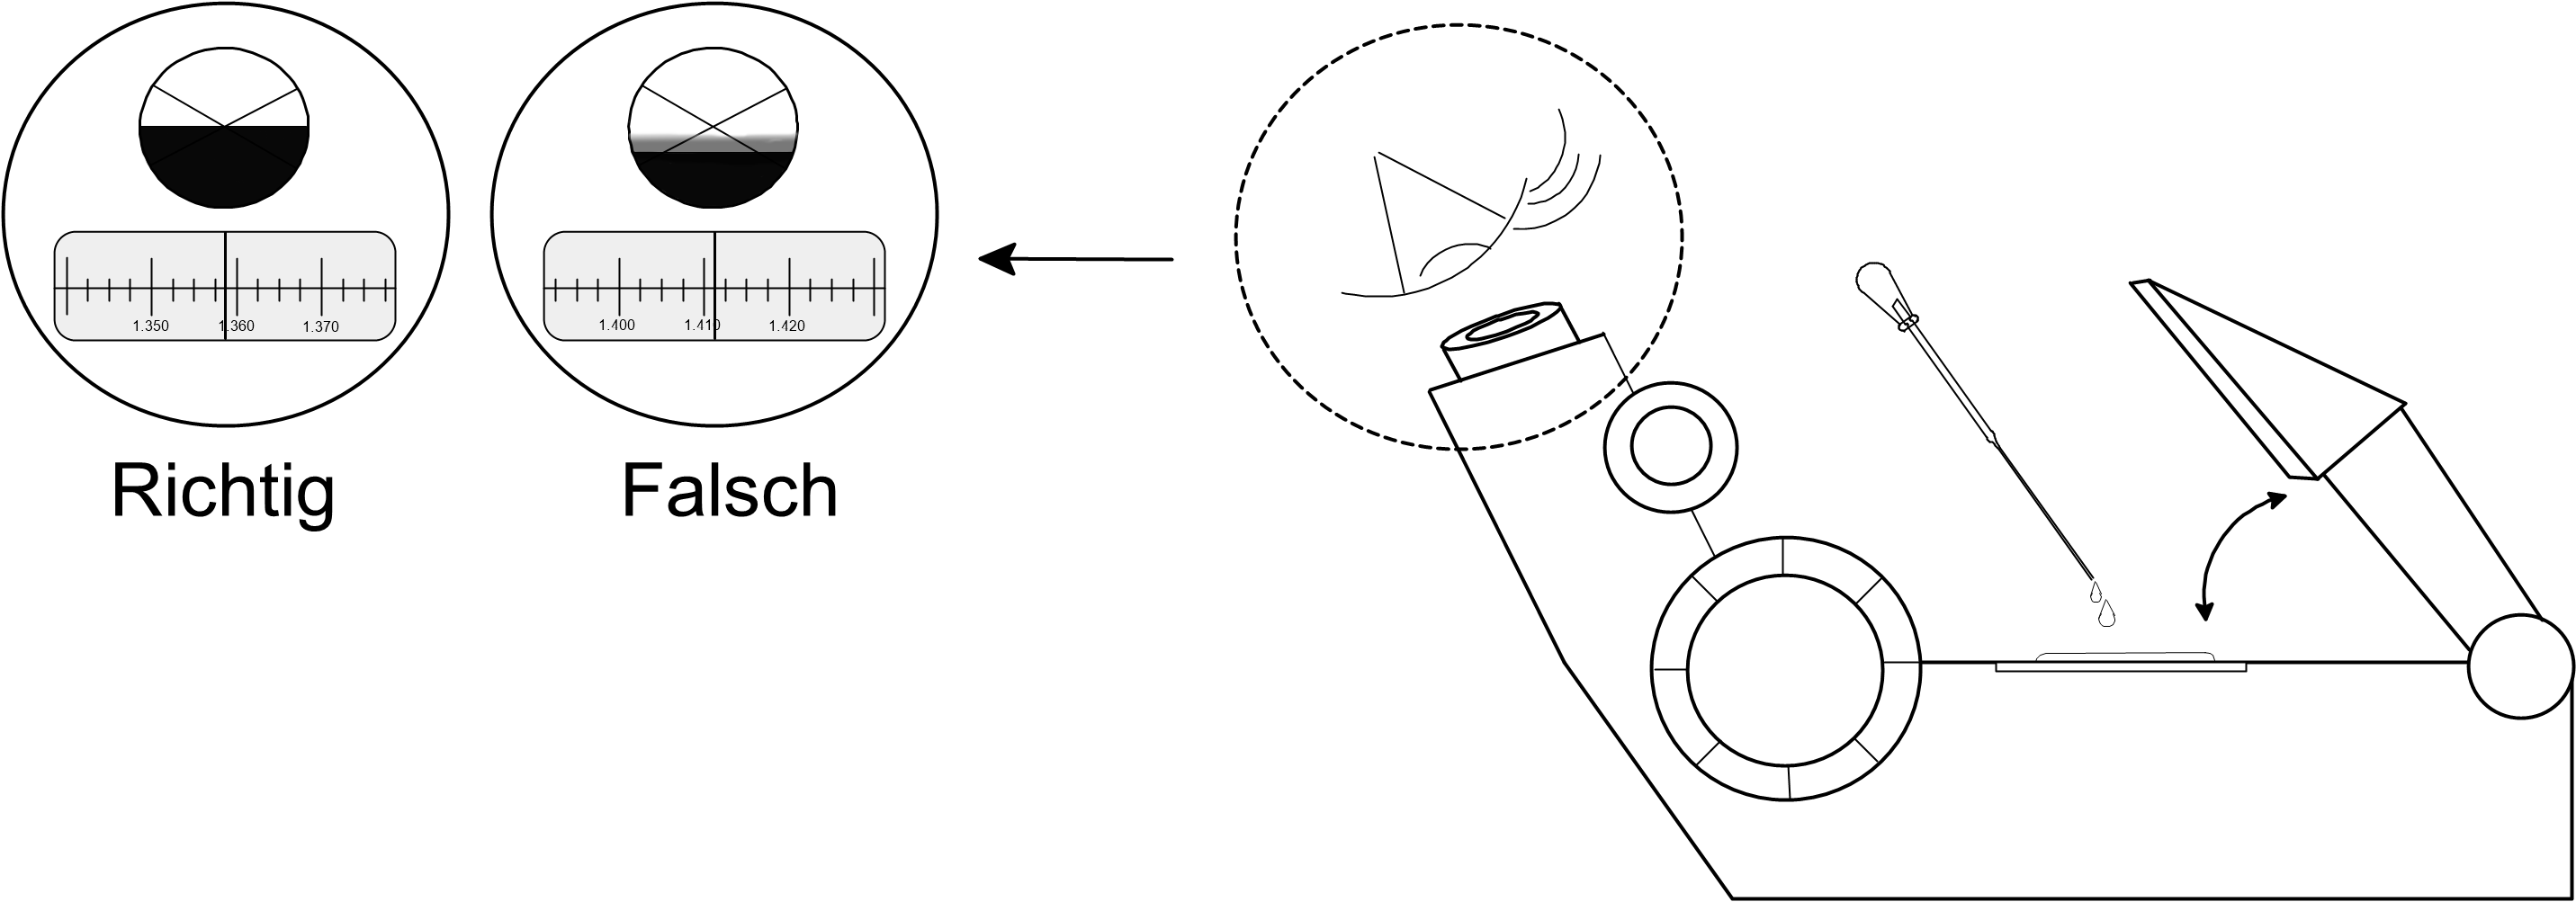
\includegraphics[width=0.75\textwidth]{img/versuchsstand/Refraktometer2}
	\caption{Brechungsindex bestimmen mit Refraktometer}
	\label{fig:refraktometrie}
\end{figure}
\FloatBarrier
%Ende

\subsubsection*{Dünnschichtchromatographie}
%Start
\begin{figure}[h!]
	\centering
	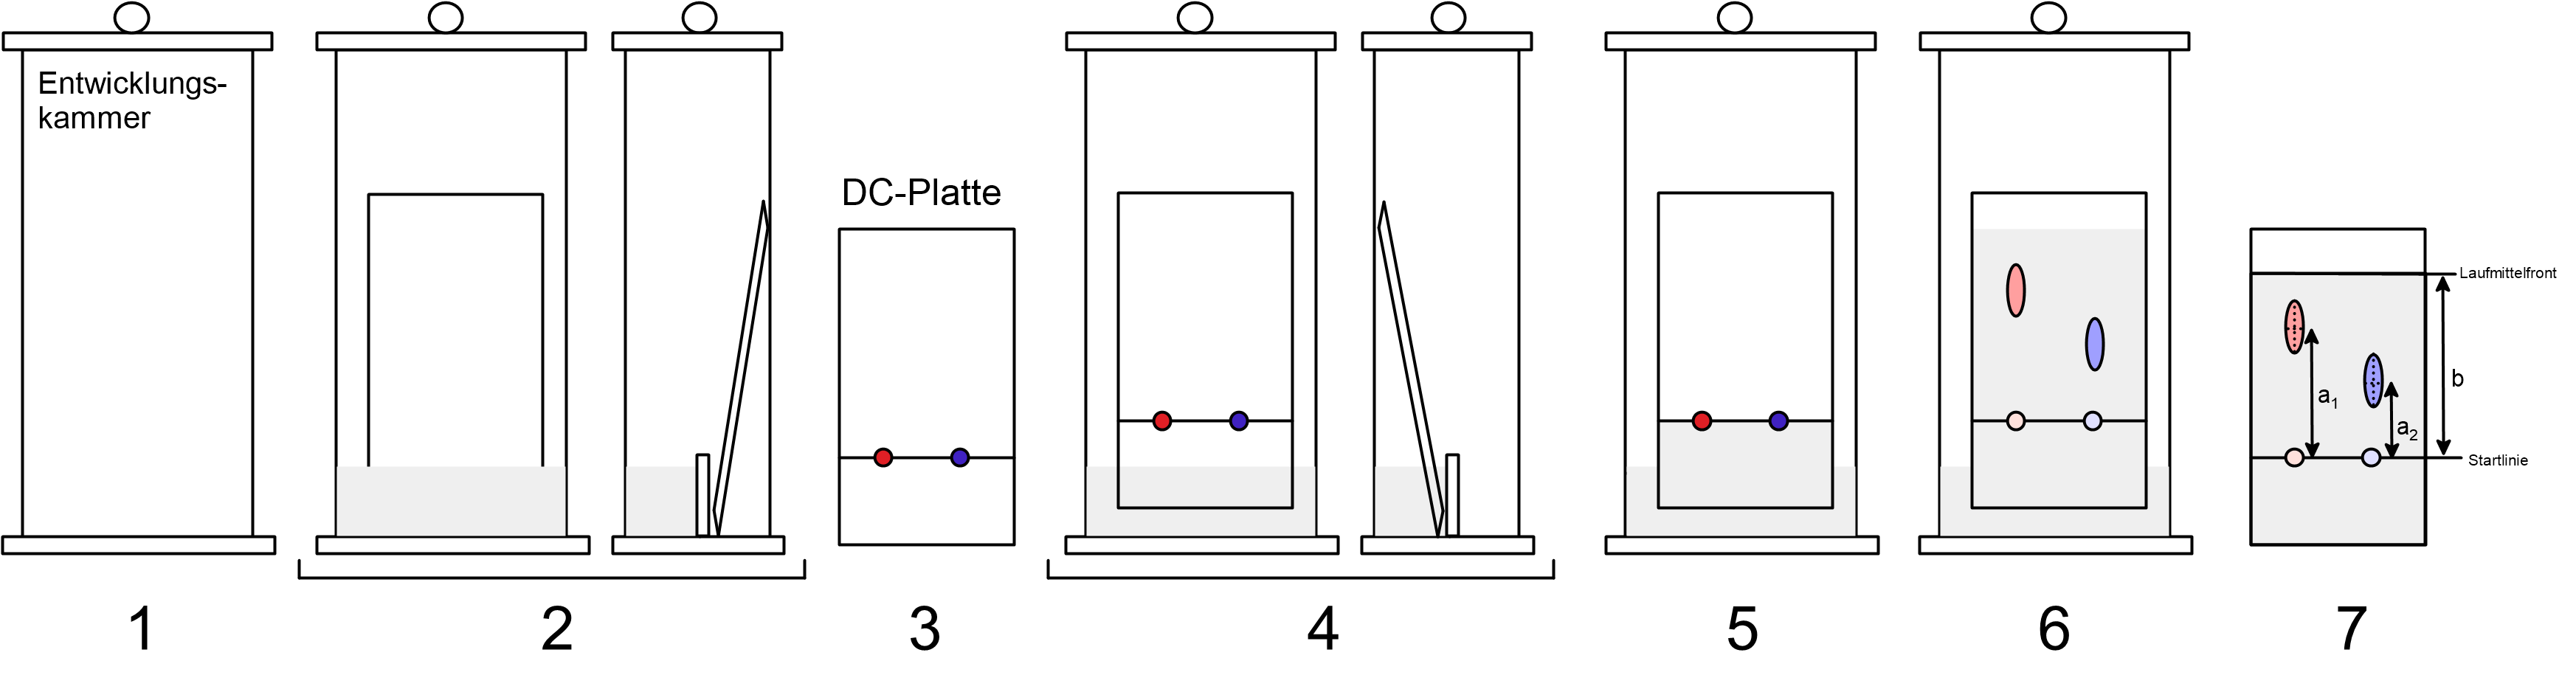
\includegraphics[width=0.85\textwidth]{img/versuchsstand/duennschicht}
	\caption{Dünnschichtchromatografie}
	\label{fig:duennschicht}
\end{figure}
\FloatBarrier
%Ende

\subsubsection*{Gaschromatografie}
%Start
\begin{figure}[h!]
	\centering
	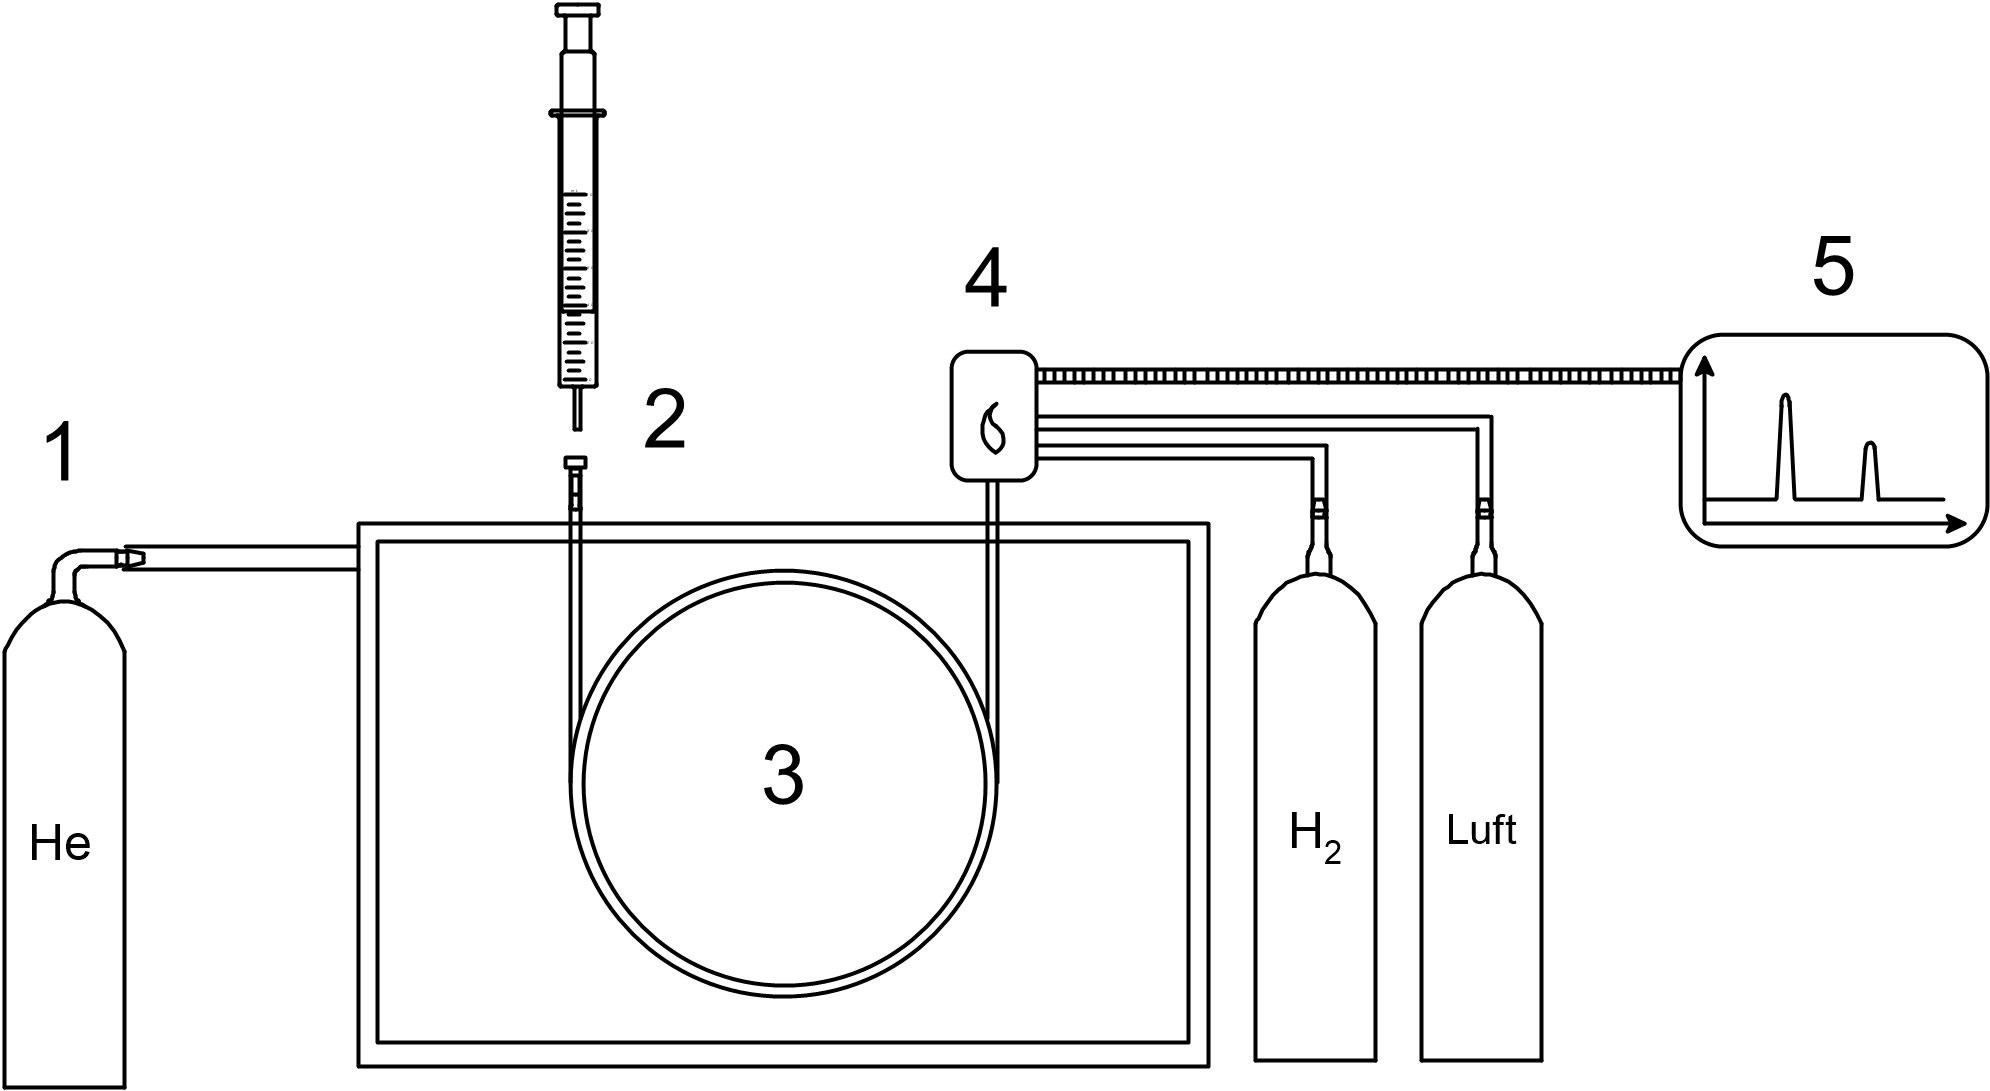
\includegraphics[width=0.6\textwidth]{img/versuchsstand/gc}
	\caption{Schematik zur Gaschromatografie}
	\label{fig:gc}
\end{figure}
\FloatBarrier
%Ende

\subsubsection*{Wasserentzug von organischen Lösungen mit Na2SO4 oder CaCl2}
%Start
\begin{figure}[h!]
	\centering
	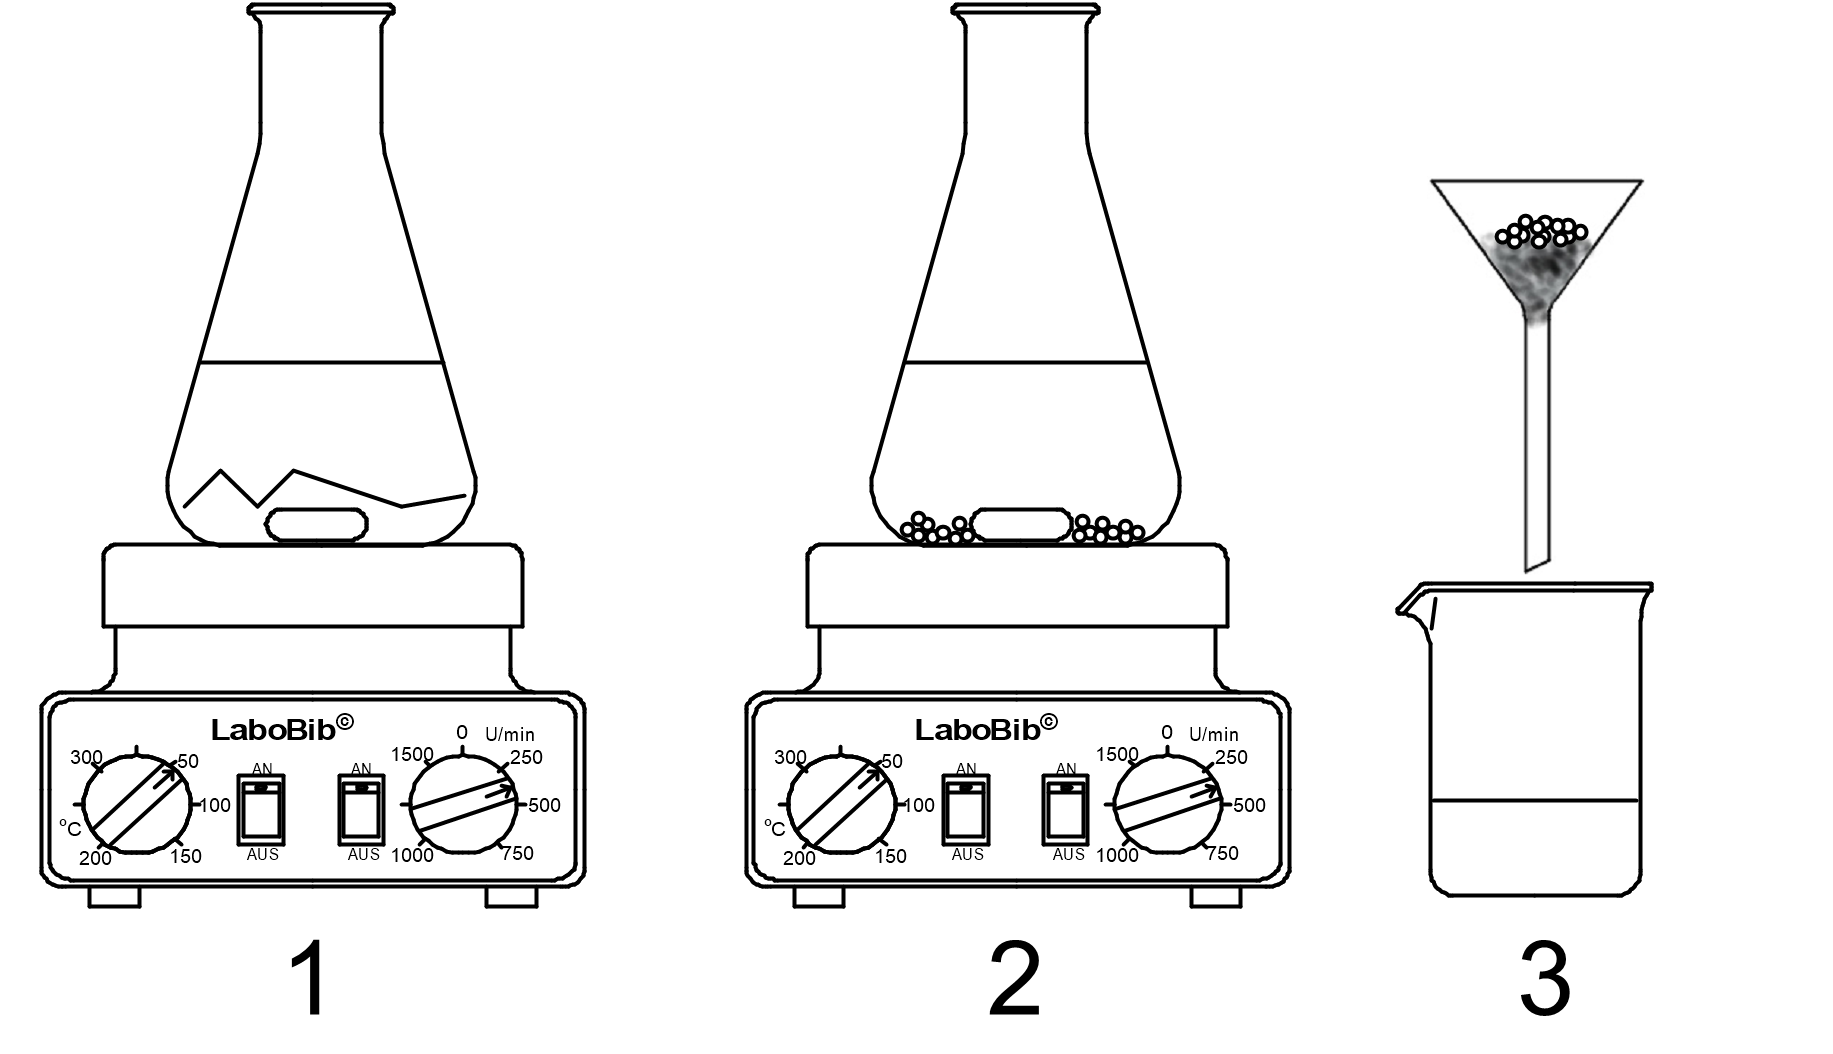
\includegraphics[width=0.6\textwidth]{img/versuchsstand/entwaessern}
	\caption{Wasserentzug aus organischen Proben}
	\label{fig:entwaessern}
\end{figure}
\FloatBarrier
%Ende